%%%%%%%%%%%%%%%%%%%%%%%%%%%%%%%%%%%%%%%%%%%%%%%%%%%%%%%%%%%%%%%%%%%%%%%%%%%%%%%
%                     Отчёт по лабораторной работе №1
%
% Дисциплина: Теория вероятностей и Математическая статистика
%                     
% Название:   Генерация выборки с различными распределениями
%
% Выполнил:   Михаил Маляренко
%
% Дата:       9 Ноя. 2020
%
%%%%%%%%%%%%%%%%%%%%%%%%%%%%%%%%%%%%%%%%%%%%%%%%%%%%%%%%%%%%%%%%%%%%%%%%%%%%%%%

% HEADER BEGIN 
\documentclass[12pt]{article}
\usepackage[utf8]{inputenc}
\usepackage[russian]{babel}
\usepackage{pscyr}
\usepackage[T2A]{fontenc}
\usepackage{geometry}
\usepackage{amsmath}
\usepackage{amssymb}
\usepackage{graphicx}
\usepackage{listings}
\usepackage{hyperref}
\usepackage{xcolor}

\geometry {	
	a4paper, 
	left   = 20mm, 
	right  = 20mm, 
	top    = 20mm, 
	bottom = 20mm
}

\definecolor{urlcolor}{HTML}{2484BC} 
\definecolor{linkcolor}{HTML}{000000}

\graphicspath{{resource/}}
% HEADER END

% DIFINES BEGIN
\newcommand{\lskip}{\hfill\break}
% DEFINES END

\begin{document}

\begin{titlepage}
	\begin{center}
		\hfill \break
		{\textbf{Санкт-Петербургский политехнический университет Петра Великого}}\\
		\hfill \break
		\textbf{Институт прикладной математики и механики}\\
		 \hfill \break
		\textbf{Кафедра <<Телематика (при ЦНИИ РТК)>>}\\
		\vfill
		\large{\bfseries Отчет по лабораторной работе}\\
		\hfill \break
		\hfill \break
		\hfill \break
		\hfill \break
		\normalsize{\bfseries Построение гистограмм по выборкам с заданным распределением}\\
		По дисциплине <<Теория вероятностей и Математическая статистика>>\\
		\hfill \break
		\hfill \break
		\hfill \break
	\end{center}
 
	\normalsize
	{ 
		\begin{tabular}{lp{2cm}cr}
			Выполнил &&&\\
			Студент гр. 3630201/80101&&\underline{\hspace{1.5cm}}& М.Д. Маляренко\\\\
			Руководитель&&&\\ 
			к.ф.-м.н., доцент && \underline{\hspace{1.5cm}}& А.Н. Баженов \\\\
			&&&<<\underline{\phantom{333}}>>\underline{\phantom{сентября000}}
			2020г.
		\end{tabular}
	}
\vfill

\begin{center} Санкт-Петербург \\2020 \end{center}
\end{titlepage}

\newpage

\setcounter{page}{2}

\begin{flushleft}

\setlength{\parindent}{1cm}

\tableofcontents

\newpage

\listoffigures

\newpage

\section{Постановка задачи}

Для заданных распределений случайных величин необходимо сгенерировать выборки из 10, 50, 1000 элементов. Для каждой выборки построить гистограмму и функцию плотности распределения вероятностей на одном графике.
\lskip

\noindentЗаданные распределения:

\begin{enumerate}
    \item Нормальное распределение $N(x, 0, 1)$
    \item Распределение Коши $C(x, 0, 1)$
    \item Распределение Лапласа $L(x, 0, 1/\sqrt{2})$
    \item Дискретное распределение Пуассона $P(k, 10)$
    \item Равномерное распределение $U(x, -\sqrt{3}, \sqrt{3})$
\end{enumerate}

\newpage

\section{Теория}

    \subsection{Рассматриваемые распределения}

        Плотности заданных распределений вероятностей \cite{theory}:

        \begin{enumerate}
            \item Нормальное распределение 
            \begin{equation}
                N(x, 0, 1) = \frac{1}{\sqrt{2\pi}}e^{-\frac{x^2}{2}}
                \label{normal}
            \end{equation}

            \item Распределение Лапласа
            \begin{equation}
                L(x, 0, 1) = \frac{1}{\pi}\frac{1}{x^2 + 1}
                \label{laplace}
            \end{equation}

            \item Распределение Коши
            \begin{equation}
                C(x, 0, 1/\sqrt{2}) =\frac{1}{\sqrt{2}} e^{-\sqrt{2}|x|}
                \label{cauchy}
            \end{equation}

            \item Дискретное распределение Пуассона
            \begin{equation}
                P(k, 10) = \frac{10^k}{k!} e^{-10}
                \label{poisson}
            \end{equation}

            \item Равномерное распределение
            \begin{equation}
                U(x, -\sqrt{3}, \sqrt{3}) = 
                \left\{
                \begin{aligned}
                    & \frac{1}{2\sqrt{3}},& \; |x| <= \sqrt{3}\\
                    & 0,                  & \; |x| >= \sqrt{3}\\
                \end{aligned}
                \right.
                \label{uniform}
            \end{equation}
        \end{enumerate}

    \subsection{Гистограмма}

        Гистограмма распределения вероятностей -- наглядное представление функции плотности вероятности случайной величины, построенное по выборке из распределения \cite{histogram}.

        Для построения гистограммы множество значений элементов выборки разбивается на интервалы, которые чаще выбираются равными, но это не обязательное условие. Гистограмма представляет собой столбчатый график, где над каждым интервалом значений элементов выборки строится столбец-прямоугольник.  При равных интервалах высота прямоугольника строится пропорционально числу элементов выборки соответсвующего интервала, при разных интервалах площадь прямоугольника пропорциональна числу элементов выборки которые попали в этот интервал.

        При выборе разбиения множества значений стоит учитывать, что существует зависимость между детализацией оценки плотности распределения, точностью её значений и количеством интервалов разбиения. В данной работе определение оптимального количества $n$ интервалов разбиения при $N = 10$ и $N = 50$ производилось эвристически, при $N = 1000$ применялась формула
        \begin{equation}
            n = \lfloor \sqrt{N} \rfloor
        \end{equation}

        При построении гистограммы распределения Пуассона каждый интервал соответствует значению дискретной случайной величины.

\newpage

\section{Реализация}

    Для построения гистограмм и графиков теоретической плотности распределения применялась система аналитических вычислений Maxima. Скрипт лабораторной работы расположен в репозитории GitHub, ссылка на который приведена в соответствующем разделе.

\newpage

\section{Результаты}

    По сгенерированным выборкам c $N = 10, 50, 1000$ случайных чисел с заданными распределениями были построены следующие графики:
    \lskip

    \noindentНа Рис. 1 представлены графики нормального распределения. Теоретическая плотность распределения вероятностей построена по формуле (\ref{normal}).

    \begin{figure}[h]
        \begin{minipage}[h]{0.325\linewidth}
            \center{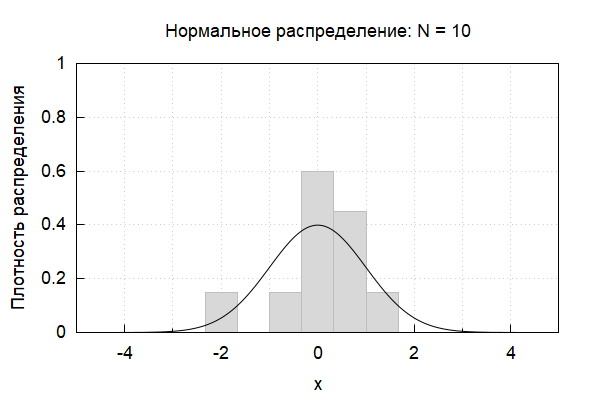
\includegraphics[width=1\linewidth]{N10.png}}
        \end{minipage}
        \begin{minipage}[h]{0.325\linewidth}
            \center{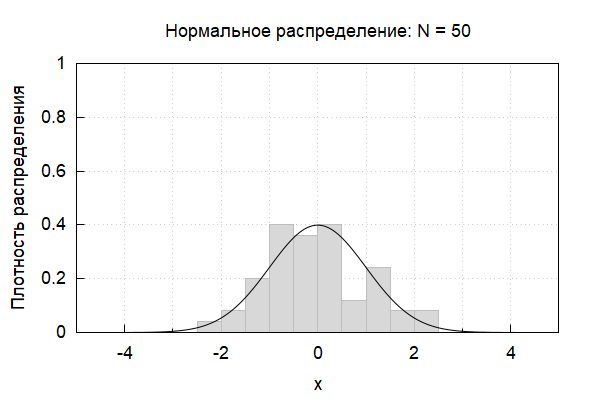
\includegraphics[width=1\linewidth]{N50.png}}
        \end{minipage}
        \begin{minipage}[h]{0.325\linewidth}
            \center{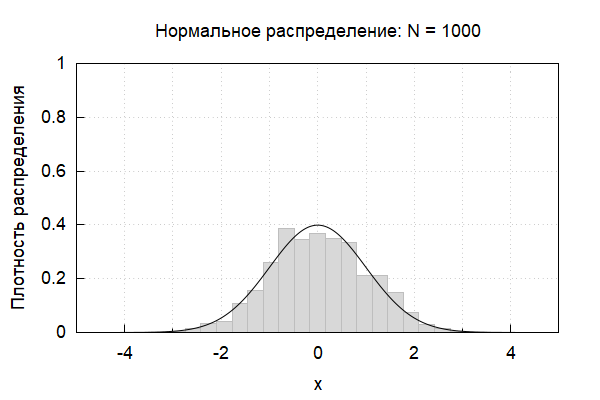
\includegraphics[width=1\linewidth]{N1000.png}}
        \end{minipage}
        \caption{Нормальное распределение $N(x, 0, 1)$}
    \end{figure}
    \lskip

    \noindentНа Рис. 2 представлены графики распределения Лапласа. Теоретическая плотность распределения вероятностей построена по формуле (\ref{laplace}).

    \begin{figure}[h!]
        \begin{minipage}[h]{0.325\linewidth}
            \center{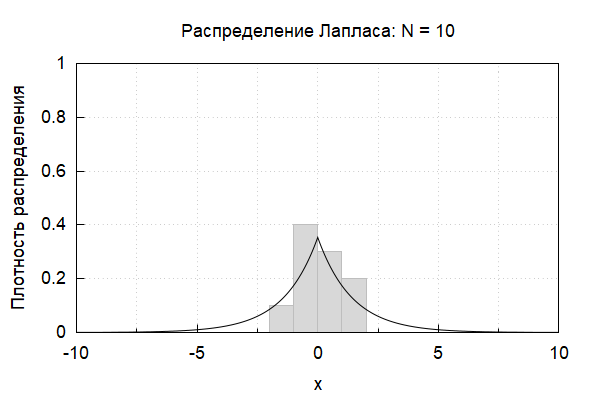
\includegraphics[width=1\linewidth]{L10.png}}
        \end{minipage}
        \begin{minipage}[h]{0.325\linewidth}
            \center{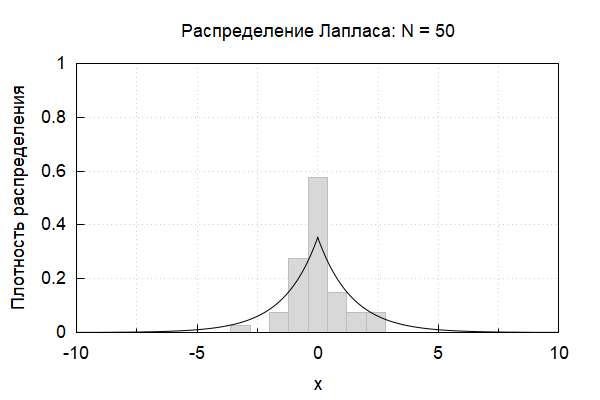
\includegraphics[width=1\linewidth]{L50.png}}
        \end{minipage}
        \begin{minipage}[h]{0.325\linewidth}
            \center{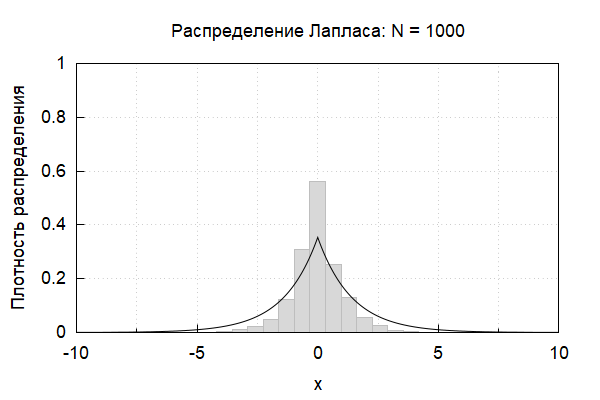
\includegraphics[width=1\linewidth]{L1000.png}}
        \end{minipage}
        \caption{Распределение Лапласа $L(x, 0, 1/\sqrt{2})$}
    \end{figure}
    \lskip

    \noindentНа Рис. 3 представлены графики распределения Коши. Теоретическая плотность распределения вероятностей построена по формуле (\ref{cauchy}).

    \begin{figure}[h!]
        \begin{minipage}[h]{0.325\linewidth}
            \center{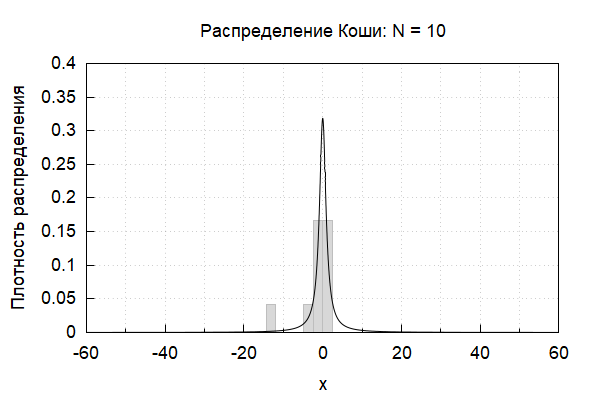
\includegraphics[width=1\linewidth]{C10.png}}
        \end{minipage}
        \begin{minipage}[h]{0.325\linewidth}
            \center{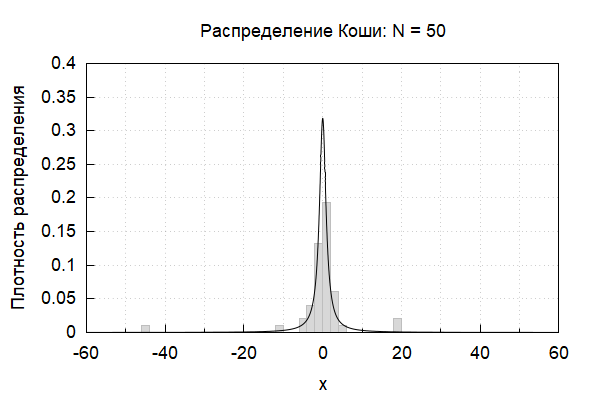
\includegraphics[width=1\linewidth]{C50.png}}
        \end{minipage}
        \begin{minipage}[h]{0.325\linewidth}
            \center{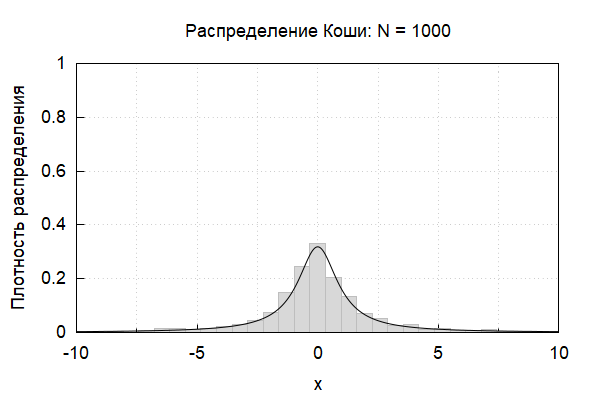
\includegraphics[width=1\linewidth]{C1000.png}}
        \end{minipage}
        \caption{Распределение Коши $C(x, 0, 1)$}
    \end{figure}

    \newpage

    \noindentНа Рис. 4 представлены графики дискретного распределения Пуассона. Теоретическая плотность распределения вероятностей построена по формуле (\ref{poisson})

    \begin{figure}[h!]
        \begin{minipage}[h]{0.325\linewidth}
            \center{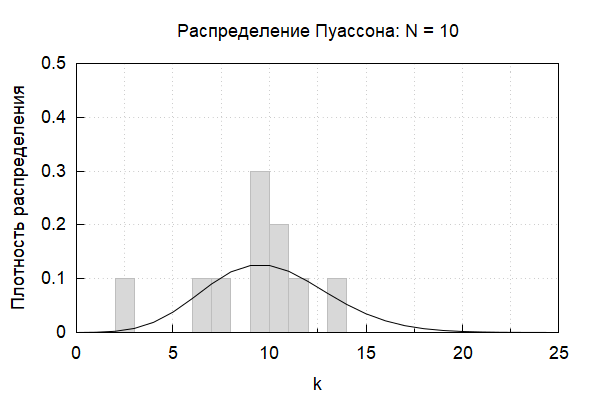
\includegraphics[width=1\linewidth]{P10.png}}
        \end{minipage}
        \begin{minipage}[h]{0.325\linewidth}
            \center{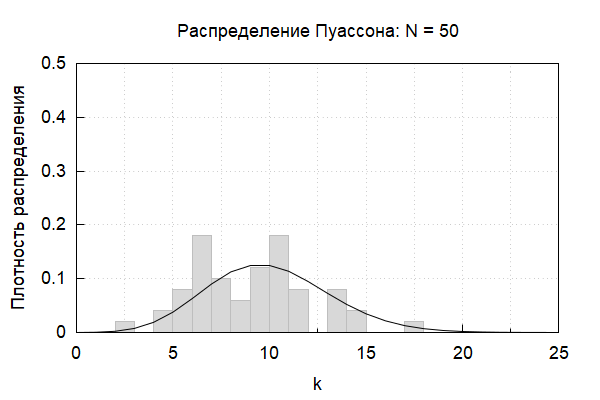
\includegraphics[width=1\linewidth]{P50.png}}
        \end{minipage}
        \begin{minipage}[h]{0.325\linewidth}
            \center{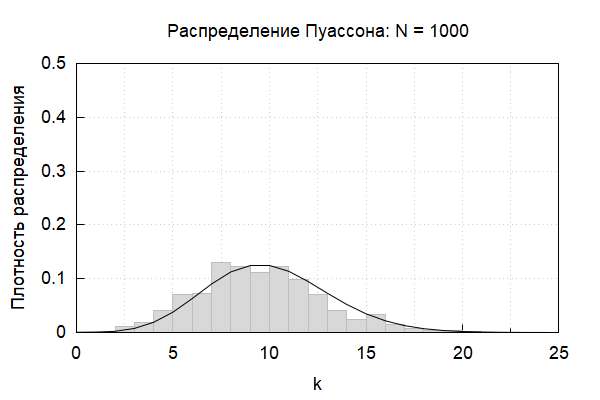
\includegraphics[width=1\linewidth]{P1000.png}}
        \end{minipage}
        \caption{Дискретное распределение Пуассона $P(k, 10)$}
    \end{figure}
    \lskip

    \noindentНа Рис. 5 представлены графики равномерного распределения. Теоретическая плотность распределения вероятностей построена по формуле (\ref{uniform})

    \begin{figure}[h!]
        \begin{minipage}[h]{0.325\linewidth}
            \center{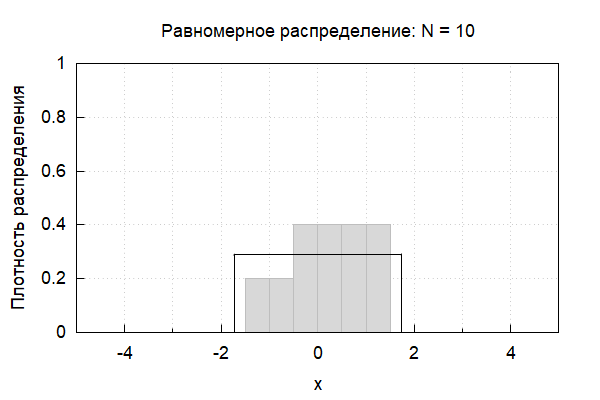
\includegraphics[width=1\linewidth]{U10.png}}
        \end{minipage}
        \begin{minipage}[h]{0.325\linewidth}
            \center{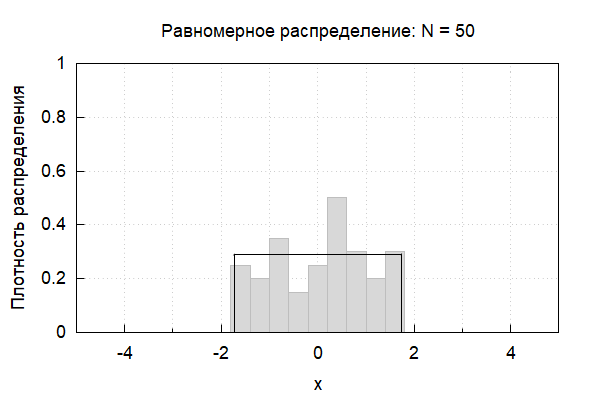
\includegraphics[width=1\linewidth]{U50.png}}
        \end{minipage}
        \begin{minipage}[h]{0.325\linewidth}
            \center{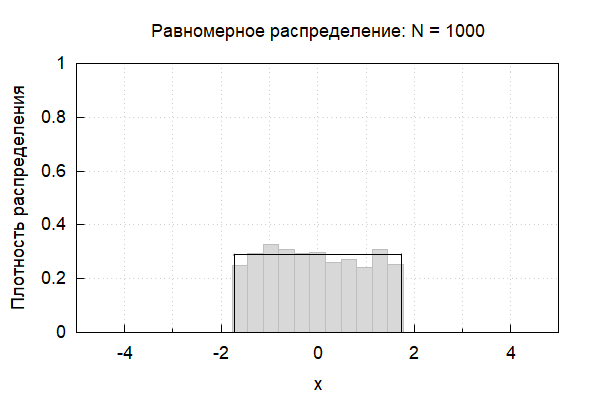
\includegraphics[width=1\linewidth]{U1000.png}}
        \end{minipage}
        \caption{Нормальное распределение $U(x, -\sqrt{3}, \sqrt{3})$}
    \end{figure}

\newpage

\section*{Заключение}
\addcontentsline{toc}{section}{Заключение}

В ходе данной лабораторной работы были сгенерированы выборки трёх размеров для пяти заданных распределений. По данным выборкам были сформированы гистограммы и они были визуально сопоставлены с теоретической плотностью распределения.

Как видно из графиков, с увеличением мощности выборки плотность распределения вероятностей приближается к своему теоретическому значению.

Для построения выборок и графиков была использована среда аналитических вычислений Maxima в связке с утилитой gnuplot.

\newpage

\addcontentsline{toc}{section}{Список литературы}

\begin{thebibliography}{9}
    \bibitem{histogram}
        Histogram \url{https://en.wikipedia.org/wiki/Histogram} Дата обращения 9.11.2020
    
        \bibitem{theory}
        Теоретическое приложение к лабораторным работам №1-4 по дисциплине «Математическая статистика». -- СПб.: СПбПУ, 2020. -- 12 c 
	
\end{thebibliography}

\newpage

\section*{Приложение А. Репозиторий с исходным кодом}
\addcontentsline{toc}{section}{Приложение А. Репозиторий с исходным кодом}

Исходный код скрипта для среды Maxima находится в репозитории GitHub -- URL \url{https://github.com/malyarenko-md/TeorVer}

\end{flushleft}

\end{document}